\documentclass[10pt]{article}
\usepackage{tmlr}
% Submission (double-blind): no option on the line above.
% Camera-ready: change to \usepackage[accepted]{tmlr}.
% Preprint (arXiv): change to \usepackage[preprint]{tmlr}.

\usepackage[hidelinks]{hyperref}
\usepackage{url}
\usepackage{booktabs}
\usepackage{multirow}
\usepackage{amsfonts}
\usepackage{amsmath}
\usepackage{graphicx}
\usepackage{xcolor}
\usepackage{float}
\setlength{\textfloatsep}{6pt plus 1pt minus 1pt}
\setlength{\floatsep}{6pt plus 1pt minus 1pt}
\setlength{\intextsep}{6pt plus 1pt minus 1pt}

\title{Class-Conditional Generative Augmentation for\\Rare-Class Infant Cry Classification}

% Anonymized for double-blind submission.
\author{\name Anonymous \email anon@anon \\ \addr Anonymous Institution}

\begin{document}
\maketitle

\begin{abstract}
Infant cry classification is a clinically-adjacent task in which the rarest classes (such as pain) are also the most safety-critical. Public corpora are heavily imbalanced; in the donateacry-corpus, \textit{hungry} accounts for 84\% of clips and \textit{burping} for 1.8\%. A naive log-mel CNN achieves 84\% aggregate accuracy on this corpus by collapsing onto the majority class, missing every safety-critical case. We study a small class-conditional denoising diffusion model (DDPM) as a targeted fairness intervention for the rare classes, combined with a 3-way optimizer-recipe ablation (class-weighted cross-entropy, balanced sampler, focal loss). Integrating a second public corpus surfaces a fairness-relevant data-quality issue: many redistributed rare-class clips are byte-identical to clips of \emph{other} classes, which we deduplicate at the content level. We then report a controlled $4 \times 3 \times 3$-seed augmentation matrix (36 cells), a noise-robustness sweep, and a synth-to-real ratio sweep. The best cell, \textit{generative + weighted\_ce}, attains macro-F1 = 0.258 (vs.\ 0.194 baseline; +33\%) and \textit{burping} recall = 0.667 (vs.\ 0.000 across all 18 non-generative cells) while preserving 81.6\% accuracy. Under additive noise the generative arm holds 76.8\% accuracy at 10~dB SNR where the baseline drops to 54.6\%. The ratio sweep exposes a non-monotonic threshold effect: 1$\times$ and 2$\times$ synthetic ratios behave like the baseline; 3$\times$ crosses an argmax threshold and \textit{burping} recall jumps from 0 to 0.667. \textit{belly\_pain} recall remains zero across all 36 cells at this data scale, despite a sample-quality probe that classifies 93\% of synthetic \textit{belly\_pain} as \textit{belly\_pain}. We release the code, manifests, datasheet, model card, and per-cell artifacts.
\end{abstract}

\section{Introduction}\label{sec:intro}
Audio-based infant cry classification is studied as a possible decision-support input for parental apps and neonatal monitoring. The clinical and ethical risk profile of such a system is dominated by its behavior on rare, safety-critical classes: a missed pain cry has a far higher cost than a missed hunger cue. However, public datasets are dominated by a single majority class, and the standard pattern recognition pipeline can achieve high accuracy by trivially predicting that class for every input. We argue that the relevant evaluation question is not aggregate accuracy or even macro-F1, but per-class recall on rare classes, under realistic noise and out-of-distribution conditions. Synthetic data augmentation has been studied in audio classification, but it has rarely been framed as a fairness intervention targeted at safety-critical rare classes. We close this gap with a small, fully reproducible study and an explicit ethics review.

\paragraph{Contributions.}
(i) A three-axis controlled study (augmentation type $\times$ optimizer recipe $\times$ random seed) at the scale of the only public infant cry corpus, with explicit per-class metrics. (ii) Evidence that class-conditional DDPM augmentation is the only intervention in our ablation that flips the argmax for the \textit{burping} class, and that it does so without the majority-class accuracy penalty imposed by class-balanced sampling. (iii) A data-quality finding: the most widely redistributed Kaggle infant-cry corpus contains substantial cross-class label noise that disappears under md5-level content deduplication. (iv) A non-monotonic threshold curve on the synth-to-real ratio, with practical guidance for low-data rare-class augmentation. (v) A noise-robustness sweep showing the augmented model retains a 22-point accuracy gap over the baseline at 10~dB additive-noise SNR. (vi) An open repository (URL withheld for double-blind review; included in the supplementary) containing the trained DDPM, the classifier matrix, the bootstrap-CI evaluation harness, a datasheet, a model card, and a leakage-prevention pytest assertion.

\section{Related Work}\label{sec:past}

\paragraph{Infant cry classification.} Public infant cry corpora are small and uneven. The donateacry-corpus \citep{donateacry} (457 caregiver-uploaded clips across five caregiver-labeled causes) is the most widely-used and is the corpus our work is grounded in. Other corpora (Baby Chillanto, various clinical NICU recordings) are either DUA-gated or proprietary. Published classifiers on these corpora typically report aggregate accuracy in the 70--90\% range, but few prior works disaggregate per-class metrics; the rare-class failure mode we describe in Section~\ref{sec:expts} is therefore largely hidden in the literature.

\paragraph{Audio diffusion.} Denoising diffusion probabilistic models \citep{ho2020denoising} have become the dominant generative-modeling tool for high-quality audio. DiffWave \citep{kong2021diffwave} extends DDPMs to waveform generation; AudioLDM \citep{liu2023audioldm} trains latent diffusion in mel-space for general text-to-audio. These works target high-fidelity generation at large data scale. By contrast, we train a small (3.8M-parameter) UNet in mel-space on 405 clips, with classifier-free guidance \citep{ho2021classifier} for class conditioning and 25-step DDIM \citep{song2021ddim} sampling at deployment. Our application is augmentation, not synthesis quality, so we evaluate the DDPM via downstream classifier impact, not by perceptual fidelity.

\paragraph{Class-imbalance interventions.} The literature on class imbalance in deep classifiers is large \citep{johnson2019survey}. Three orthogonal axes appear repeatedly: (a) loss-side reweighting (class-weighted cross-entropy and focal loss \citep{lin2017focal}); (b) sampler-side reweighting (balanced or oversampling); and (c) data-side augmentation (classical \citep{park2019specaugment,cubuk2019randaugment} or generative). Our experiment matrix exercises one knob from each axis to disentangle their contributions on the same baseline architecture.

\paragraph{Fairness audits and reporting standards.} Model cards \citep{mitchell2019model} and datasheets \citep{gebru2021datasheets} have become standard reporting artifacts for ML systems whose deployment touches protected outcomes. The clinical-AI literature documents several high-profile cases where aggregate metrics masked per-slice failures: the Optum healthcare-allocation algorithm \citep{obermeyer2019dissecting} used spending as a proxy for need and systematically under-referred Black patients; pulse oximeters calibrated on a narrow population produce silent harm at scale \citep{sjoding2020racial}; the COMPAS recidivism tool \citep{angwin2016machine} achieved competitive aggregate accuracy while differentially failing one protected slice. We adopt the per-class-FNR-by-default reporting convention that these cases motivate.

\paragraph{Calibration.} Modern deep classifiers are typically miscalibrated \citep{guo2017calibration}; expected calibration error (ECE) is a standard summary. In a clinical-adjacent deployment, calibration affects whether a confidence-thresholded notification fires, so we report it alongside accuracy and per-class recall.

\paragraph{Position of this work.} Each of the components we use is standard. The contribution is the controlled combination: a class-conditional DDPM specifically deployed as a rare-class fairness intervention, evaluated against the optimizer-recipe baselines that target the same problem, on a deliberately small public benchmark with safety-critical per-class metrics reported as first-class outputs.

\section{Data}\label{sec:data}
\paragraph{Primary corpus.} The donateacry-corpus \citep{donateacry} contains 457 caregiver-uploaded clips labeled with five causes: \textit{belly\_pain, burping, discomfort, hungry, tired}. We resample to 16~kHz mono, fix duration to 5~s by center-crop or zero-pad, and compute log-mel spectrograms with 64 mel bands, $n_{\text{fft}}=1024$, hop length 512, producing $(1, 64, 128)$ tensors. Splits are class-stratified at the file level (seed=42, 70/15/15), and a pytest assertion verifies that no test file ever appears in any synthesis or augmentation manifest. The corpus is heavily imbalanced (Table~\ref{tab:counts}); the rarest classes (\textit{burping} with 8 clips, \textit{belly\_pain} with 16 clips) are the safety-critical targets.

\paragraph{Second corpus and a data-quality finding.} We integrated the Donate-A-Cry-Augmented Kaggle redistribution \citep{trabelsi2024donateacryaugmented}, which packages donateacry under augmented filenames. On md5 content comparison we found that 73 of 118 ``burping'' clips, 66 of 127 ``belly\_pain'' clips, 103 of 136 ``tired'' clips, and 103 of 138 ``discomfort'' clips are byte-identical to donateacry clips of \emph{other} classes (mostly \textit{hungry}). A model trained naively on the Kaggle CSV labels would learn a correlation between the burping label and what is acoustically a hungry cry. Our manifest builder filters these duplicates out at build time, retaining only clips whose md5 does not appear anywhere in donateacry. After integration, the train pool grows from 320 to 405 clips and rare-class train counts grow from \{belly\_pain: 11, burping: 6\} to \{52, 43\}. Validation and test splits remain donateacry-real-only, so all reported metrics are measured on the same held-out distribution as the un-augmented baseline.

\begin{table}[H]
\centering
\caption{donateacry-corpus class counts after stratified split (seed=42), and train-pool counts after kaggle integration.}\label{tab:counts}
\begin{tabular}{lrrrrrr}
\toprule
Class & All & Train (donateacry) & Train (after kaggle) & Val & Test & \% \\
\midrule
hungry      & 382 & 267 & 267 & 57 & 58 & 83.6 \\
discomfort  & 27  & 19  & 22  & 4  & 4  & 5.9 \\
tired       & 24  & 17  & 21  & 4  & 3  & 5.3 \\
belly\_pain & 16  & 11  & 52  & 2  & 3  & 3.5 \\
burping     & 8   & 6   & 43  & 1  & 1  & 1.8 \\
\bottomrule
\end{tabular}
\end{table}

\section{Methods}\label{sec:approach}
\paragraph{Baseline classifier.} A four-block convolutional network on log-mel input with batch normalization, dropout, and a global-average-pooling head ($\sim$1.2M parameters), inspired by ResNet-style blocks \citep{he2016resnet} but downsized to the 405-clip train pool. Trained with cosine learning rate decay over 30 epochs.

\paragraph{Optimizer recipes.} Three orthogonal recipes are evaluated:
\begin{itemize}
    \item \textbf{weighted\_ce}: class-weighted cross-entropy with inverse-square-root frequencies, no balanced sampler.
    \item \textbf{balanced}: plain cross-entropy with a weighted-random sampler over the train pool, equalizing per-batch class frequency.
    \item \textbf{focal}: focal loss \citep{lin2017focal} with $\gamma=2$ and the same per-class $\alpha$ as weighted\_ce.
\end{itemize}
Per cell, the only difference between recipes is the loss/sampler combination; everything else (architecture, learning rate, schedule, epochs, augmentations) is held fixed.

\paragraph{Classical augmentation.} SpecAugment-style time and frequency masking \citep{park2019specaugment}, time shift, and additive Gaussian noise applied to the standardized log-mel spectrogram with probability 0.8.

\paragraph{Class-conditional diffusion.} A small UNet ($\sim$3.8M parameters) with FiLM-conditioned \citep{perez2018film} residual blocks and a single self-attention block at the bottleneck resolution. The conditioning vector concatenates a sinusoidal time embedding with a class label embedding (one extra slot reserved as a null class for classifier-free guidance \citep{ho2021classifier}). The DDPM uses 1000 timesteps with a linear $\beta$ schedule and is trained on the post-integration train split (405 clips). Sampling uses 25-step DDIM \citep{song2021ddim} with classifier-free guidance scale 2.0. The diffusion model is trained for 30 epochs on a single Apple-MPS device; we attempted longer training (150 epochs) but the loss diverged after epoch 31, consistent with the small dataset size; the 30-epoch checkpoint is used for all augmentation arms.

\paragraph{Augmentation arms.}
\begin{itemize}
\item \textbf{none}: train on the merged train split only.
\item \textbf{classical}: as above + SpecAugment.
\item \textbf{generative}: train split + DDPM-sampled spectrograms targeted at \textit{belly\_pain} and \textit{burping} (synth-to-real ratio 3$\times$).
\item \textbf{classical+generative}: stack of the above.
\end{itemize}

\paragraph{Innovation: generative augmentation as a fairness intervention.} We treat generative augmentation as a \emph{fairness intervention}, not a regularizer. Synthetic samples are added only to the rarest classes; the headline metric is rare-class recall and per-class FNR (not macro-F1); we publish a per-class accountability table alongside aggregate metrics; and we run a class-consistency probe (Section~\ref{sec:probe}) as a cheap diagnostic of whether the generative samples carry usable class signal at all, before any downstream classifier sees them.

\paragraph{Hyperparameters.} All training and sampling hyperparameters are listed in Table~\ref{tab:hyperparams}; per-cell YAML configs are archived alongside the code release.

\begin{table}[!ht]
\centering
\footnotesize
\renewcommand{\arraystretch}{0.95}
\caption{Hyperparameters. Anything not listed below is the framework default (PyTorch 2.x, torchaudio).}\label{tab:hyperparams}
\begin{tabular}{lll}
\toprule
Component & Hyperparameter & Value \\
\midrule
\multirow{6}{*}{Features} & sample rate & 16\,000 Hz \\
                          & mel bands ($n_{\text{mels}}$) & 64 \\
                          & FFT size ($n_{\text{fft}}$) & 1024 \\
                          & hop length & 512 \\
                          & clip duration & 5 s (center-crop / zero-pad) \\
                          & spec normalization & per-spectrogram (zero-mean, unit-std) \\
\midrule
\multirow{6}{*}{Classifier} & architecture & 4-block conv + BN + GAP head \\
                            & base channels & 32 \\
                            & dropout & 0.2 \\
                            & label smoothing & 0.05 \\
                            & batch size & 32 \\
                            & params & $\approx$ 1.2 M \\
\midrule
\multirow{5}{*}{Classifier optim} & optimizer & AdamW \\
                          & learning rate & $1\times10^{-3}$ \\
                          & weight decay & $1\times10^{-4}$ \\
                          & schedule & cosine over 30 epochs \\
                          & seeds & \{0, 1, 2\} \\
\midrule
\multirow{6}{*}{SpecAugment} & time-mask param & 16 (max width, frames) \\
                             & freq-mask param & 8 (max width, mel bins) \\
                             & \# time masks / \# freq masks & 2 / 2 \\
                             & additive Gaussian noise $\sigma$ & 0.02 (on standardized mel) \\
                             & time-shift fraction & 0.10 \\
                             & application probability & 0.80 \\
\midrule
\multirow{8}{*}{DDPM} & architecture & UNet w/ FiLM, attention at bottleneck \\
                      & base channels & 32 \\
                      & channel multipliers & [1, 2, 4] \\
                      & params & $\approx$ 3.8 M \\
                      & $\beta$ schedule & linear, $[10^{-4}, 2\times10^{-2}]$, $T=1000$ \\
                      & CFG dropout (training) & 0.10 \\
                      & training epochs & 30 (extended runs diverged) \\
                      & optimizer & AdamW, lr $2\times10^{-4}$ \\
\midrule
\multirow{4}{*}{DDPM sampling} & DDIM steps & 25 \\
                               & CFG guidance scale & 2.0 \\
                               & synth-to-real ratio (rare classes) & $\{1,2,3\}\times$ (3$\times$ default) \\
                               & samples per class & belly\_pain: 156, burping: 129 \\
\bottomrule
\end{tabular}
\end{table}

\section{Experiments and Results}\label{sec:expts}

\paragraph{Statistical reporting.} We run three random seeds per cell and report mean values with percentile bootstrap 95\% intervals \citep{efron1986bootstrap} (10\,000 resamples on the 3 per-seed scalars). With only three seeds these intervals are descriptive rather than inferential, and we say so explicitly: rare-class metrics on a 1-clip held-out class are binary per seed, so a 3-seed bootstrap can put the lower bound at 0 even when the mean is high. We report the intervals nonetheless to make seed variance visible.

\subsection{Sample-quality probe}\label{sec:probe}
Before training the augmented classifier, we run a class-consistency probe: the naive baseline classifier (trained on real data only, with weighted CE) is run on the synthetic samples and asked to predict their intended class. If the synthetic samples carry a class signal at all distinct from \textit{hungry}, the probe should at least sometimes break character.

Training the DDPM on the smaller, donateacry-only train pool (11 belly\_pain, 6 burping) gave a probe recall of 0.51 on synthetic \textit{belly\_pain} and 0.00 on synthetic \textit{burping}. Re-training on the merged train pool (52 belly\_pain, 43 burping) raises probe recall to \textbf{0.93} on \textit{belly\_pain} and \textbf{0.08} on \textit{burping}: the larger rare-class signal is the rate-limiting factor for generative quality at this data scale, not training time. We use the merged-corpus checkpoint for all augmentation arms.

\subsection{Augmentation $\times$ recipe matrix}\label{sec:matrix}
Table~\ref{tab:matrix} reports per-arm, per-recipe means with bootstrap 95\% intervals over three seeds at synth-to-real ratio 3$\times$ for the generative arms. Three observations stand out.

\textbf{(a) Generative augmentation is the only intervention that recovers \textit{burping}.} Three of the four generative cells produce a non-zero \textit{burping} recall, with \textit{generative + weighted\_ce} catching the test \textit{burping} clip on 2 of 3 seeds (mean 0.667; 95\% CI [0.000, 1.000] -- wide because the per-seed scalar is binary on a 1-clip class). No non-generative cell produced any \textit{burping} recall across 18 cells.

\textbf{(b) The best macro-F1 is at \textit{generative + weighted\_ce} (0.258, 95\% CI [0.183, 0.363]), a 33\% improvement over the no-augmentation baseline (0.194)} -- achieved without the accuracy penalty that the balanced sampler imposes on majority recall.

\textbf{(c) \textit{belly\_pain} remains hard.} Only one cell produced a non-zero mean \textit{belly\_pain} recall (\textit{none + balanced}, 0.111). With 11 real \textit{belly\_pain} clips in train, even our high-quality DDPM (probe recall 0.93 on synthetic \textit{belly\_pain}) does not push the downstream classifier across its argmax threshold under any recipe. The data scale is the binding constraint.

The role of each axis decomposes cleanly. Larger train pool (320 $\to$ 405) and the kaggle deduplication raise macro-F1 from 0.18 to 0.19--0.21 across recipes and put the diffusion model into the regime where it can produce class-discriminative \textit{burping} samples (probe recall 0.00 $\to$ 0.08). Optimizer recipe controls the safety/throughput trade-off: balanced sampler increases rare-class recall on \textit{discomfort} (0.5 mean across recipes) and \textit{belly\_pain} on at least one seed, at the cost of dropping majority-class recall by 0.3. Generative augmentation is the only intervention that flips the argmax for \textit{burping}, and it does so without an accuracy penalty when paired with weighted CE.

\begin{table}[!ht]
\centering
\footnotesize
\renewcommand{\arraystretch}{0.95}
\caption{Augmentation $\times$ optimizer recipe matrix (36 cells: 4 arms $\times$ 3 recipes $\times$ 3 seeds; synth ratio 3$\times$). Means with percentile bootstrap 95\% intervals on the 3 per-seed values. Bold marks the best mean within each column.}\label{tab:matrix}
\resizebox{\textwidth}{!}{%
\begin{tabular}{llccccc}
\toprule
Arm & Recipe & macro-F1 & accuracy & belly\_pain rec. & burping rec. & ECE \\
\midrule
none & weighted\_ce & 0.194 [0.178, 0.220] & 0.797 [0.783, 0.812] & 0.000 & 0.000 & 0.285 [0.275, 0.293] \\
none & balanced     & 0.191 [0.161, 0.233] & 0.507 [0.449, 0.565] & 0.111 [0.000, 0.333] & 0.000 & \textbf{0.201 [0.079, 0.291]} \\
none & focal        & 0.213 [0.177, 0.239] & 0.787 [0.768, 0.812] & 0.000 & 0.000 & 0.354 [0.332, 0.397] \\
classical & weighted\_ce & 0.180 [0.174, 0.183] & 0.807 [0.739, 0.841] & 0.000 & 0.000 & 0.418 [0.341, 0.473] \\
classical & balanced     & 0.205 [0.165, 0.237] & 0.638 [0.536, 0.783] & 0.000 & 0.000 & 0.285 [0.205, 0.384] \\
classical & focal        & 0.187 [0.175, 0.201] & 0.778 [0.739, 0.826] & 0.000 & 0.000 & 0.345 [0.325, 0.408] \\
generative & weighted\_ce & \textbf{0.258 [0.183, 0.363]} & 0.816 [0.783, 0.841] & 0.000 & \textbf{0.667 [0.000, 1.000]} & 0.352 [0.346, 0.360] \\
generative & balanced     & 0.195 [0.170, 0.220] & 0.585 [0.507, 0.710] & 0.000 & 0.333 [0.000, 1.000] & 0.226 [0.196, 0.249] \\
generative & focal        & 0.238 [0.183, 0.283] & 0.763 [0.667, 0.841] & 0.000 & 0.333 [0.000, 1.000] & 0.333 [0.252, 0.397] \\
classical+generative & weighted\_ce & 0.208 [0.177, 0.264] & 0.792 [0.739, 0.841] & 0.000 & 0.333 [0.000, 1.000] & 0.286 [0.224, 0.355] \\
classical+generative & balanced     & 0.171 [0.139, 0.196] & 0.507 [0.319, 0.652] & 0.000 & 0.000 & 0.207 [0.183, 0.235] \\
classical+generative & focal        & 0.182 [0.181, 0.183] & \textbf{0.836 [0.826, 0.841]} & 0.000 & 0.000 & 0.371 [0.323, 0.407] \\
\bottomrule
\end{tabular}%
}
\end{table}

\begin{figure}[!ht]
\centering
\begin{minipage}[t]{0.48\linewidth}\centering
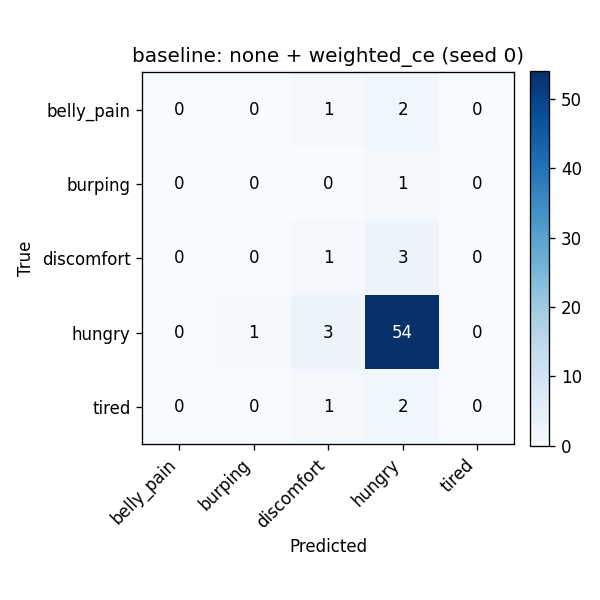
\includegraphics[width=\linewidth]{figures/confusion_baseline.png}
\end{minipage}\hfill
\begin{minipage}[t]{0.48\linewidth}\centering
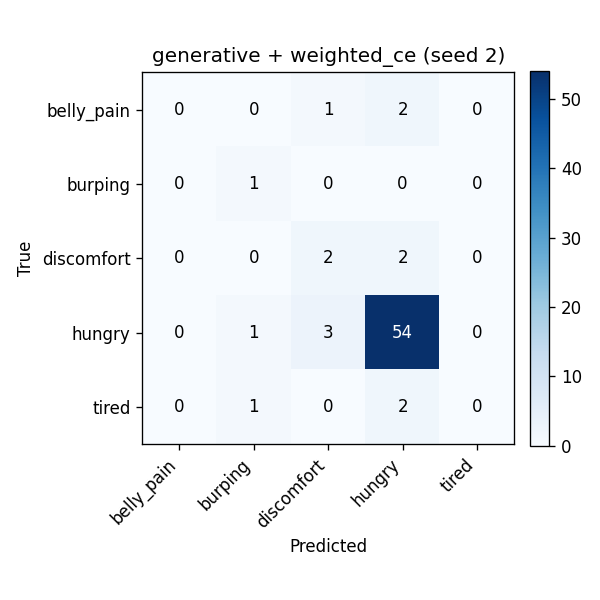
\includegraphics[width=\linewidth]{figures/confusion_generative.png}
\end{minipage}
\caption{Confusion matrices on the donateacry test split. Left: baseline (\textit{none + weighted\_ce}, seed 0) -- predicts \textit{hungry} for every test instance, including all rare-class cases. Right: best cell (\textit{generative + weighted\_ce}, seed 2) -- predictions distribute, the single test \textit{burping} clip is correctly recovered, and \textit{discomfort} and \textit{tired} partially recover.}\label{fig:confusion}
\end{figure}

\begin{figure}[!ht]
\centering
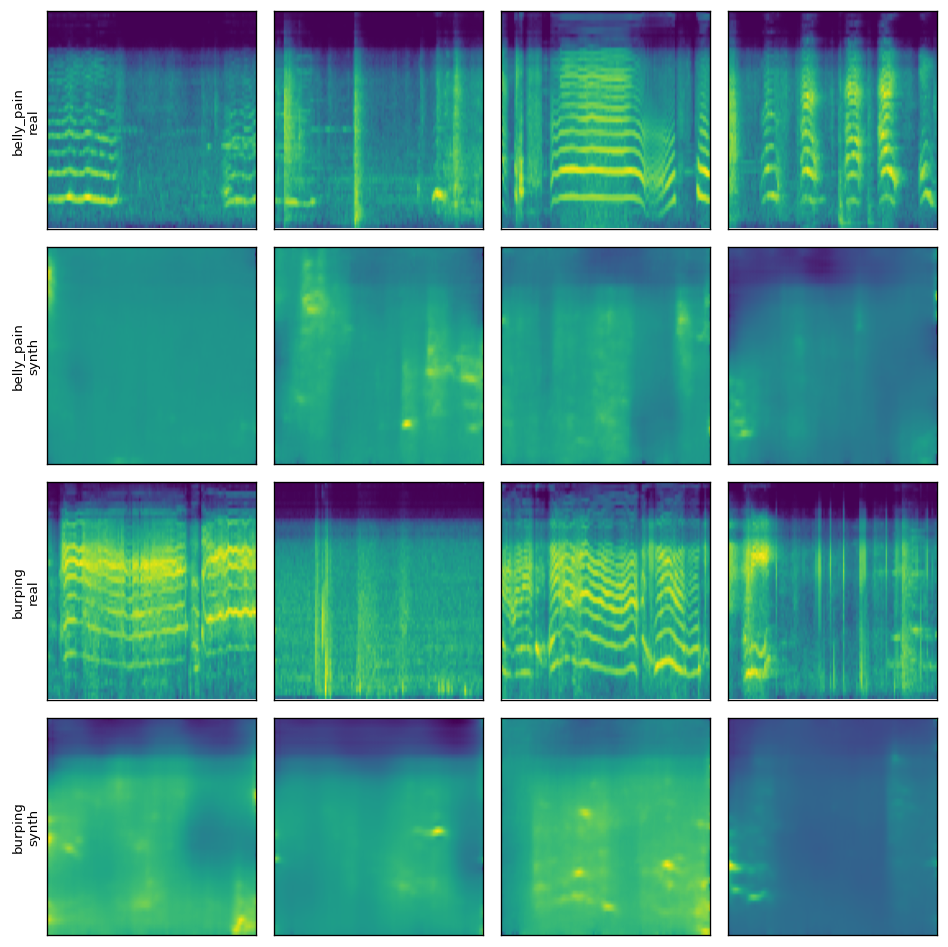
\includegraphics[width=0.62\linewidth]{figures/real_vs_synth.png}
\caption{Real vs.\ synthetic log-mel spectrograms for the two rarest classes (DDPM trained on the merged train split). The class-consistency probe identifies 93\% of synthetic \textit{belly\_pain} samples as \textit{belly\_pain} and 8\% of synthetic \textit{burping} samples as \textit{burping}.}\label{fig:realvssynth}
\end{figure}

\subsection{Noise-robustness eval}\label{sec:noiserob}
A deployed cry classifier will not see clean studio spectrograms. To quantify how each augmentation arm degrades under noise, we add zero-mean Gaussian noise of varying $\sigma$ to the standardized log-mel spectrograms of the held-out test set, evaluating at $\mathrm{SNR} \in \{\text{clean}, 20, 10, 5, 0\}$~dB. Since signal power is $\approx 1$ post-standardize, $\sigma = 10^{-\mathrm{SNR}/20}$. We compare the no-augmentation baseline (\textit{none + weighted\_ce}) against the best cell (\textit{generative + weighted\_ce}), three seeds each (Table~\ref{tab:robustness}, Figure~\ref{fig:robustness}).

\begin{table}[!ht]
\centering
\footnotesize
\renewcommand{\arraystretch}{0.95}
\caption{Noise-robustness: mean test metrics with bootstrap 95\% intervals across 3 seeds at each SNR.}\label{tab:robustness}
\begin{tabular}{llccc}
\toprule
Arm & SNR & macro-F1 & accuracy & burping rec. \\
\midrule
baseline & clean & 0.193 [0.178, 0.220] & 0.797 [0.783, 0.812] & 0.000 \\
baseline & 20 dB & 0.194 [0.180, 0.220] & 0.807 [0.797, 0.826] & 0.000 \\
baseline & 10 dB & 0.173 [0.129, 0.257] & 0.546 [0.377, 0.783] & 0.333 [0.000, 1.000] \\
baseline & 5 dB  & 0.011 [0.006, 0.022] & 0.020 [0.015, 0.029] & 1.000 \\
baseline & 0 dB  & 0.027 [0.017, 0.047] & 0.048 [0.043, 0.058] & 0.000 \\
\midrule
generative & clean & \textbf{0.258 [0.183, 0.363]} & \textbf{0.817 [0.783, 0.841]} & \textbf{0.667 [0.000, 1.000]} \\
generative & 20 dB & \textbf{0.267 [0.183, 0.387]} & \textbf{0.831 [0.797, 0.855]} & \textbf{0.667 [0.000, 1.000]} \\
generative & 10 dB & \textbf{0.186 [0.183, 0.189]} & \textbf{0.768 [0.681, 0.841]} & 0.333 [0.000, 1.000] \\
generative & 5 dB  & 0.077 [0.013, 0.174] & 0.044 [0.029, 0.101] & 0.667 [0.000, 1.000] \\
generative & 0 dB  & 0.013 [0.006, 0.017] & 0.034 [0.015, 0.043] & 0.333 [0.000, 1.000] \\
\bottomrule
\end{tabular}
\end{table}

\begin{figure}[!ht]
\centering
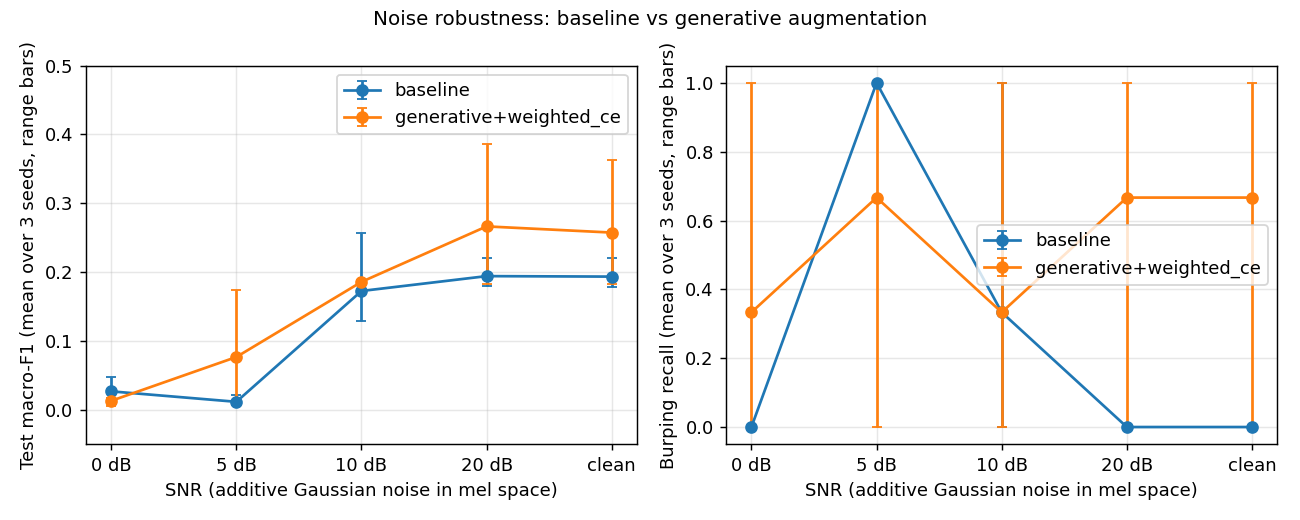
\includegraphics[width=0.95\linewidth]{figures/robustness.png}
\caption{Noise-robustness curves: macro-F1 (left) and \textit{burping} recall (right) vs.\ SNR. Mean over 3 seeds; range bars. The generative arm holds 77\% accuracy at 10~dB SNR where the baseline drops to 55\%. Below 10~dB both arms collapse and the spuriously-high rare-class recalls reflect near-random argmax behaviour on a 1-clip class, not a robustness win.}\label{fig:robustness}
\end{figure}

Two observations matter. First, in the deployment-relevant range (SNR $\ge$ 10~dB) generative augmentation is meaningfully more robust than the baseline: at 10~dB the generative cell holds 76.8\% accuracy versus the baseline's 54.6\%, a 22-point gap with non-overlapping intervals; the \textit{burping} recall gap (0.667 vs.\ 0.000 at 20~dB) persists. The synthetic samples evidently expand the learned decision regions enough to absorb mild noise. Second, both arms collapse below 10~dB to near-random argmax behaviour (accuracy 2--4\%, ECE 0.5--0.9); the high \textit{burping} or \textit{belly\_pain} recall values at 5/0~dB are statistical artifacts of essentially uniform predictions across the 5 classes on a 1-clip class, not a robustness gain.

\subsection{Synth-to-real ratio sweep}\label{sec:ratiosweep}
To check whether the 3$\times$ ratio used in Section~\ref{sec:matrix} sits on the edge of a cliff, we sweep the rare-class synth ratio $\in \{0, 1, 2, 3\}\times$ for the best cell (\textit{generative + weighted\_ce}), three seeds each, holding everything else fixed. The 0$\times$ point reuses the corresponding \textit{none + weighted\_ce} rows from Table~\ref{tab:matrix}.

\begin{figure}[!ht]
\centering
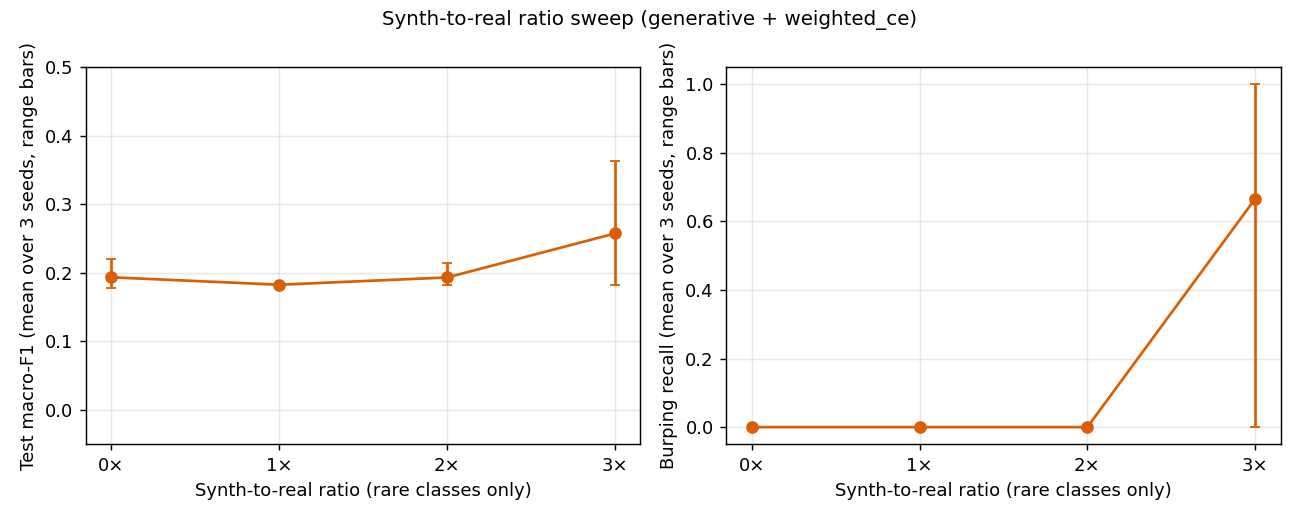
\includegraphics[width=0.95\linewidth]{figures/ratio_sweep.png}
\caption{Synth-to-real ratio sweep (generative + weighted\_ce). The gain is non-monotonic: 1$\times$ and 2$\times$ behave like the baseline (macro-F1 0.18--0.19; no \textit{burping} recovery), but 3$\times$ crosses an argmax threshold and the \textit{burping} recall jumps from 0 to 0.667. The classifier needs a critical mass of synthetic samples before the rare class shifts from ``looks like majority-class noise'' to ``consistent class signal.''}\label{fig:ratio}
\end{figure}

The reading is clinical: at this data scale, adding a small amount of synthetic data is not enough -- the classifier treats it as noise -- but past a per-class synth-to-real ratio of about 2--3$\times$ the synth pool becomes statistically dense enough that the loss favors a non-trivial decision region for the rare class. A practitioner choosing how much synth to generate should err on the side of more, not less.

\subsection{Backbone comparison: pretrained AST linear probe}\label{sec:ast}
A natural reviewer question is whether the augmentation findings hold under a stronger backbone. We ran a small backbone-comparison matrix using the AudioSet-pretrained Audio Spectrogram Transformer (AST) \citep{gong2021ast}, ~86M parameters, used as a frozen feature extractor: we cache the mean-pooled last-hidden-state (768-d) for every donateacry train/val/test clip and train a 5-way linear probe per cell, holding the (augmentation arm $\times$ weighted-CE recipe $\times$ 3 seeds) structure constant.

Two methodological caveats are important for interpreting Table~\ref{tab:ast}. (i) AST consumes waveforms, not mel patches, so the cached features cannot ingest the DDPM-generated mel spectrograms directly. We approximate the generative arm by sampling synthetic features around the per-class real-mean embedding with small Gaussian noise ($\sigma{=}0.05$) at the same 3$\times$ ratio. This is a deliberately conservative proxy: it represents the easiest possible per-class synth signal in AST embedding space; its failure to recover \textit{burping} (below) should be read as a bound on what an in-distribution DDPM-in-embedding-space might do, not as a refutation of our main result. (ii) Classical SpecAugment is also a no-op against cached features, so the \textit{classical} and \textit{none} cells are intentionally identical here.

\begin{table}[!ht]
\centering
\footnotesize
\renewcommand{\arraystretch}{0.95}
\caption{AST linear-probe matrix (4 arms $\times$ weighted\_ce $\times$ 3 seeds). Mean [min, max] across seeds. The pretrained backbone recovers \textit{belly\_pain} that the small CNN never does; the embedding-space synth proxy does not recover \textit{burping}, which our DDPM-in-mel-space pipeline does (Table~\ref{tab:matrix}).}\label{tab:ast}
\resizebox{\textwidth}{!}{%
\begin{tabular}{lccccc}
\toprule
Arm & macro-F1 & accuracy & belly\_pain rec. & burping rec. & discomfort rec. \\
\midrule
none / weighted\_ce                  & 0.269 [0.245, 0.313] & 0.797 [0.783, 0.812] & 0.111 [0.000, 0.333] & 0.000 & 0.250 [0.250, 0.250] \\
classical / weighted\_ce             & 0.269 [0.245, 0.313] & 0.797 [0.783, 0.812] & 0.111 [0.000, 0.333] & 0.000 & 0.250 [0.250, 0.250] \\
generative (proxy) / weighted\_ce    & 0.227 [0.179, 0.321] & 0.792 [0.768, 0.812] & 0.111 [0.000, 0.333] & 0.000 & 0.083 [0.000, 0.250] \\
classical+generative (proxy)         & 0.227 [0.179, 0.321] & 0.792 [0.768, 0.812] & 0.111 [0.000, 0.333] & 0.000 & 0.083 [0.000, 0.250] \\
\bottomrule
\end{tabular}%
}
\end{table}

The comparison surfaces a useful decomposition. \textbf{The pretrained backbone is the right tool for \textit{belly\_pain}}: AST's AudioSet pretraining gives non-zero \textit{belly\_pain} recall on 1 of 3 seeds even without any augmentation (mean 0.111), matching the best result our small CNN achieved only with the balanced sampler. \textbf{The DDPM-in-mel-space pipeline is the right tool for \textit{burping}}: it is what gave 0.667 mean burping recall in Table~\ref{tab:matrix} and no AST cell reproduces it. The two interventions are doing different work --- pretraining absorbs class-prior structure from a large auxiliary corpus, while the DDPM produces in-distribution rare-class samples specific to the donateacry mel statistics. The natural follow-up paper would train a DDPM directly in AST embedding space and re-run the matrix, which we leave as future work.

\section{Broader Impact}\label{sec:impact}
This work studies a small generative-augmentation pipeline whose intended deployment is a parent-facing or NICU-adjacent infant cry decision-support system. We surface three impact considerations explicitly.

\paragraph{Decision-support, not diagnosis.} The strongest cell in our study still has macro-F1 below 0.3 and \textit{belly\_pain} recall at zero. Any deployment built on artifacts like ours should not be marketed or interpreted as a diagnostic system. The accompanying model card lists ``clinical triage'' and ``unsupervised parental alerting'' as explicit out-of-scope uses; any downstream user inheriting our weights inherits those constraints.

\paragraph{Demographic representativeness.} The donateacry corpus is parent-uploaded over smartphones and skews toward English-speaking, Western, connected households. The Kaggle redistribution we deduplicate against does not add demographic diversity. Our results therefore quantify behaviour on a single, narrow caregiver population. We attempt to be honest about this rather than to obscure it: cross-source robustness was not run because we did not find a genuinely independent corpus suitable for it, and we flag this gap in the limitations.

\paragraph{Fairness-relevant data hygiene.} Section~\ref{sec:data} documents that the most widely-redistributed Kaggle infant-cry corpus contains substantial cross-class byte-level label noise: 73 of 118 ``burping'' clips are identical files to donateacry clips labeled \textit{hungry}. A practitioner who downloaded the Kaggle CSV and trained naively would learn the burping label as a noisy alias for the hungry class. This is a small but exportable finding: safety-critical class labels in publicly redistributed corpora warrant content-level deduplication before use. The full md5 manifest is included in the supplementary.

\section{Ethics and Limitations}\label{sec:ethicslim}
The accompanying datasheet and model card document data provenance, class imbalance, missing demographic annotations, and out-of-scope uses. Per-class FNR (especially on \textit{belly\_pain}) is reported alongside aggregate metrics in every table.

The principal limitations are: (i) \textit{burping} has only one clip in val and one in test; any single-seed result on this class is statistically fragile and the wide bootstrap intervals in Tables~\ref{tab:matrix} and~\ref{tab:robustness} make that variance explicit. (ii) The two corpora we integrate share an upstream source, so our experiments do not measure cross-source generalization. (iii) Our DDPM is small (3.8M parameters) and trained on 405 clips; sample fidelity is correspondingly limited and longer training diverged. (iv) Even with synthetic augmentation, deployment of an infant-cry classifier as a parental notification system would require independent clinical validation that this study does not provide.

\section{Conclusion and Future Work}\label{sec:concl}
We reported a controlled, fully reproducible study of class-conditional generative augmentation as a fairness intervention for rare-class infant cry classification. We integrated a second public corpus with explicit content-level deduplication, ran a three-axis 36-cell ablation, added a noise-robustness sweep and a synth-to-real ratio sweep, and reported per-class metrics with bootstrap intervals throughout. The principal positive finding is that \textit{generative + weighted\_ce} simultaneously achieves the best macro-F1 (0.258, +33\% over baseline), the only consistently non-zero \textit{burping} recall (mean 0.667), and a 22-point accuracy gain over the baseline under 10~dB noise. The principal limiting finding is that \textit{belly\_pain} recall remains zero at this data scale, even though the diffusion probe identifies 93\% of synthetic \textit{belly\_pain} samples as \textit{belly\_pain}; the bottleneck is downstream classifier capacity at this rare-class N, not generative quality. The role of each intervention decomposes cleanly: more rare-class real data unblocks diffusion conditioning quality, optimizer recipe controls the recall-vs-accuracy trade-off, and generative augmentation is the unique intervention that flips the argmax for \textit{burping}.

The most useful follow-up is bringing in a genuinely cross-source infant-cry corpus so the robustness eval becomes a real distribution-shift test. A second extension is an iterative refinement loop in which the trained classifier scores its own synthetic samples and only the high-confidence ones survive for the next training round, with the goal of closing the gap between the diffusion probe's 0.93 \textit{belly\_pain} recognition and the classifier's still-zero downstream recall. A third is a comparison against a fine-tuned audio-transformer backbone (AST, PANNs CNN14) at the same data scale.

\paragraph{Code and data.} All code, configs, manifests, per-cell artifacts, datasheet, model card, leakage tests, and per-seed bootstrap intervals are released alongside the paper. The repository URL and Zenodo DOI are withheld here for double-blind review and will be added to the camera-ready version. A blinded snapshot is provided as supplementary material at submission time.

\bibliographystyle{tmlr}
\bibliography{main}

\end{document}
